\documentclass[a4paper, 11pt]{article}\usepackage[]{graphicx}\usepackage[]{color}
% maxwidth is the original width if it is less than linewidth
% otherwise use linewidth (to make sure the graphics do not exceed the margin)
\makeatletter
\def\maxwidth{ %
  \ifdim\Gin@nat@width>\linewidth
    \linewidth
  \else
    \Gin@nat@width
  \fi
}
\makeatother

\definecolor{fgcolor}{rgb}{0.345, 0.345, 0.345}
\newcommand{\hlnum}[1]{\textcolor[rgb]{0.686,0.059,0.569}{#1}}%
\newcommand{\hlstr}[1]{\textcolor[rgb]{0.192,0.494,0.8}{#1}}%
\newcommand{\hlcom}[1]{\textcolor[rgb]{0.678,0.584,0.686}{\textit{#1}}}%
\newcommand{\hlopt}[1]{\textcolor[rgb]{0,0,0}{#1}}%
\newcommand{\hlstd}[1]{\textcolor[rgb]{0.345,0.345,0.345}{#1}}%
\newcommand{\hlkwa}[1]{\textcolor[rgb]{0.161,0.373,0.58}{\textbf{#1}}}%
\newcommand{\hlkwb}[1]{\textcolor[rgb]{0.69,0.353,0.396}{#1}}%
\newcommand{\hlkwc}[1]{\textcolor[rgb]{0.333,0.667,0.333}{#1}}%
\newcommand{\hlkwd}[1]{\textcolor[rgb]{0.737,0.353,0.396}{\textbf{#1}}}%
\let\hlipl\hlkwb

\usepackage{framed}
\makeatletter
\newenvironment{kframe}{%
 \def\at@end@of@kframe{}%
 \ifinner\ifhmode%
  \def\at@end@of@kframe{\end{minipage}}%
  \begin{minipage}{\columnwidth}%
 \fi\fi%
 \def\FrameCommand##1{\hskip\@totalleftmargin \hskip-\fboxsep
 \colorbox{shadecolor}{##1}\hskip-\fboxsep
     % There is no \\@totalrightmargin, so:
     \hskip-\linewidth \hskip-\@totalleftmargin \hskip\columnwidth}%
 \MakeFramed {\advance\hsize-\width
   \@totalleftmargin\z@ \linewidth\hsize
   \@setminipage}}%
 {\par\unskip\endMakeFramed%
 \at@end@of@kframe}
\makeatother

\definecolor{shadecolor}{rgb}{.97, .97, .97}
\definecolor{messagecolor}{rgb}{0, 0, 0}
\definecolor{warningcolor}{rgb}{1, 0, 1}
\definecolor{errorcolor}{rgb}{1, 0, 0}
\newenvironment{knitrout}{}{} % an empty environment to be redefined in TeX

\usepackage{alltt}

\usepackage{amsmath} % e.g. for \text{} in math
\usepackage{bm}
\usepackage[T1]{fontenc}
\usepackage{geometry}
  \geometry{verbose,tmargin=2cm,bmargin=2cm,lmargin=3cm,rmargin=2cm}
  \setcounter{secnumdepth}{3}
  \setcounter{tocdepth}{3}
\usepackage{hanging}
\usepackage[utf8]{inputenc}
%\usepackage{listings}
%  \lstset{breaklines=true, showstringspaces=false}
\usepackage{natbib}
  \PassOptionsToPackage{hyphens}{url}
\usepackage[unicode=true,pdfusetitle,
 bookmarks=true,bookmarksnumbered=true,bookmarksopen=true,bookmarksopenlevel=2,
 breaklinks=true,pdfborder={0 0 1},colorlinks=false, hidelinks]{hyperref}
\usepackage{mathptmx} % for Times-compatible math font; needs to go before other font packages!
\usepackage[ttscale=.85]{libertine}
	%	\renewcommand\familydefault{\sfdefault} 
\usepackage{microtype}
\usepackage{titlesec} % for titleformat
\usepackage[nottoc]{tocbibind} % include reference in table of content
\usepackage{wrapfig}
\usepackage[dvipsnames]{xcolor}

\renewcommand{\textfraction}{0.05}
\renewcommand{\topfraction}{0.8}
\renewcommand{\bottomfraction}{0.8}
\renewcommand{\floatpagefraction}{0.75}

\renewcommand{\vec}[1]{\mathbf{#1}}                   % replaces the arrow over vectors by bold-print

\frenchspacing % avoid long spaces after a "."
\IfFileExists{upquote.sty}{\usepackage{upquote}}{}
\begin{document}

% If you HERE, after the "begin document" see something like "sweave-concordance", then you used sweave rather than knitr for processing this document. 
% In RStudio, under Options/Sweave, set to "knitr"!



\title{
\normalfont \normalsize 
\huge Consequences of changing \emph{this} for \emph{that} \\ % The assignment title
}

\author{Jo Friend (Matriculation No. 53637383)\\MSc Environmental Science\\University of Freiburg, Germany}

\maketitle

\tableofcontents


\begin{abstract}
A template to get started with writing a report weaving text and R-code.
\end{abstract}


\section{Introduction}
Reproducible statistical analysis means to make each step transparent. One approach weaves R-code into a \LaTeX\/ document, using the functionality of the \textbf{knitr} package by Yihui Xie. For help and documentation and examples see \url{https://yihui.org/knitr/}.

When you develop code, you trial a lot of code lines. Only some of them will make it into the final project document. It is thus common to work with two different R-scripts, one ending in .R, the pure R-code, and one ending in .Rnw, the project documentation. While you can do the .R in any R-editor, .Rnw are best processed in RStudio, which has a dedicated button to press (or Ctrl/Cmd-Shift-k) for compiling, which is a treat! I assume here that we use RStudio for both.

The R-code is evaluated in the console, while the project file is processed \emph{independently} in the background. That can be confusing, as the objects in the console are \emph{not} available to the document. It takes a bit of getting used to this parallel working. One option is to work only in R until, say, 2 hours before the end of the working day, then switch to the .Rnw-document and step-by-step copy-paste the relevant bits into it, and write the accompanying text. 


\section{Task 1}
When using R-code in knitr-mode, one can provide a lot of options. For example, the options `fig.height' and `fig.width' refer to the size of a figure in R, while `out.height' and `out.width' are for the eventual size in the \LaTeX\/ document.

To use R within the document, you have to start and end with a special formatting. Start the chunk with \texttt{$<< >>=$} and end with \texttt{@}. The first entry is the name of the code chunk, if you want to name it. Like this:
\begin{knitrout}\small
\definecolor{shadecolor}{rgb}{0.969, 0.969, 0.969}\color{fgcolor}\begin{kframe}
\begin{alltt}
\hlkwd{data}\hlstd{(sleep)}
\hlkwd{attach}\hlstd{(sleep)}
\hlkwd{boxplot}\hlstd{(extra} \hlopt{~} \hlstd{group,} \hlkwc{col}\hlstd{=}\hlstr{"grey"}\hlstd{,} \hlkwc{las}\hlstd{=}\hlnum{1}\hlstd{,} \hlkwc{ylab}\hlstd{=}\hlstr{"extra hours of sleep"}\hlstd{,}
          \hlkwc{xlab}\hlstd{=}\hlstr{"type of sleeping drug"}\hlstd{)}
\end{alltt}
\end{kframe}

{\centering 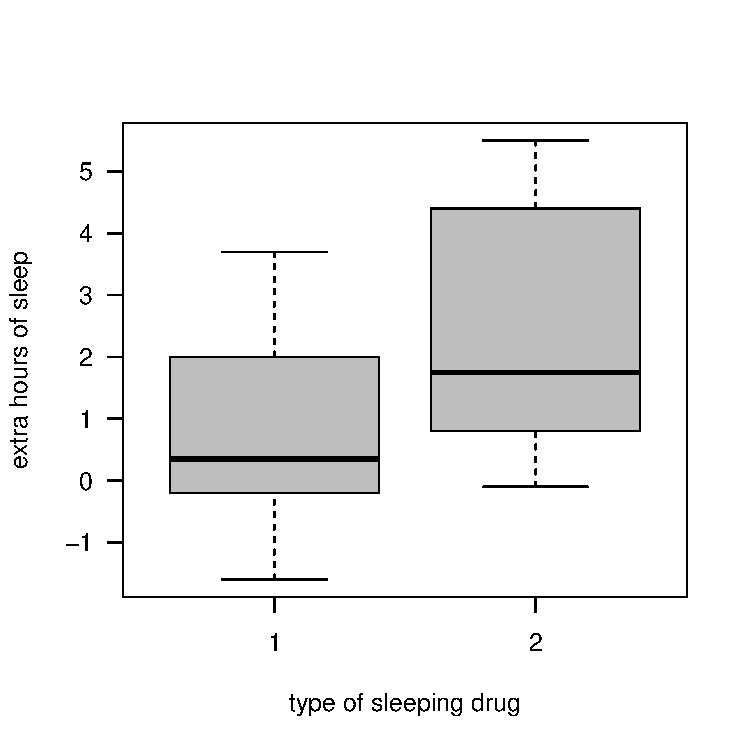
\includegraphics[width=7cm,height=7cm]{figure/example1-1} 

}



\end{knitrout}

There are many options when defining an R-chunk. Important options are:
\begin{itemize}
\item \texttt{eval=T/F} specifies whether the code is actually evaluate, i.e. computed and returned. If you only want to show but not evaluate the code, set it to false.
\item \texttt{echo=T/F} specifies whether this code chunk is actually shown in the document. We will next see a case where you want to hide the code.
\item \texttt{message=T/F} suppresses messages, such as when loading a package or attaching (and thereby overwriting) a table repeatedly.
\item \texttt{cache=T/F} tells R to store the results of a code chunk (or not). This is rather important! If you were to re-evaluate each chunk every time you add code, you would have to wait endlessly for the results. Hence, R stores the results of each chunk. But now imagine you change something in chunk 12 but chunk 14 would need to be re-evaluated, as it depends on chunk 12. This would not happen, by default, as each chunk is stored without reference to which chunk it depends on. By setting for chunk 14 \texttt{cache=F}, we can force R to evaluate a chunk every time. Use prudently!
\end{itemize}

Normally, the results of an R-chunk are stored. Thus, when you write new text, and new chunks, there should be no need to think of anything, just type. Somehow, this is not always the case. 

Imagine running some code takes 5 hours. We developed the code in the .R-file and don't want to re-run the entire 5 hours again after copy-pasting it into the .Rnw-file. Instead, we would rather store the results from the console, and, when compiling the document, \textbf{not} evaluate this chunk, and instead load the object saved.

This is how to do it: 
\begin{enumerate}
\item During your code development phase, save the file into the same folder as your document (or preferably into a subfolder, e.g. ``storedObjects''): \nolinkurl{save(myobject, file="storedObjects/myobject.Rdata")}
\item In your document, copy-paste the R-code used to generate the object into an R-chunk, but set the option \texttt{eval=F}. This chunk is now ignored in R, but set appropriately in \LaTeX.
\item Add a new chunk to load the stored object, setting the option \texttt{echo=F} to suppress it being rendered in the document: \nolinkurl{load("storedObjects/myobject.Rdata")}. This will make \texttt{myobject} available to this and further chunks.


\end{enumerate}

So, in the .R-file, we created some object \texttt{fm} which we then stored in the working directory as \texttt{sleepfm.Rdata}. This is the code how to proceed in the .Rnw-document (obviously, you cannot see this in the PDF, only in the .Rnw file!!):

\begin{knitrout}\small
\definecolor{shadecolor}{rgb}{0.969, 0.969, 0.969}\color{fgcolor}\begin{kframe}
\begin{alltt}
\hlstd{fm} \hlkwb{<-} \hlkwd{lm}\hlstd{(extra} \hlopt{~} \hlstd{group,} \hlkwc{data}\hlstd{=sleep)}
\hlstd{fm_nochmal} \hlkwb{<-} \hlkwd{lm}\hlstd{(extra} \hlopt{~} \hlstd{group,} \hlkwc{data}\hlstd{=sleep)}
\end{alltt}
\end{kframe}
\end{knitrout}

\vspace{-2\baselineskip} % to remove the white space created by the non-echoed chunk
\begin{knitrout}\small
\definecolor{shadecolor}{rgb}{0.969, 0.969, 0.969}\color{fgcolor}\begin{kframe}
\begin{alltt}
\hlkwd{summary}\hlstd{(fm)}
\end{alltt}
\begin{verbatim}
## 
## Call:
## lm(formula = extra ~ group, data = sleep)
## 
## Residuals:
##    Min     1Q Median     3Q    Max 
## -2.430 -1.305 -0.580  1.455  3.170 
## 
## Coefficients:
##             Estimate Std. Error t value Pr(>|t|)  
## (Intercept)   0.7500     0.6004   1.249   0.2276  
## group2        1.5800     0.8491   1.861   0.0792 .
## ---
## Signif. codes:  0 '***' 0.001 '**' 0.01 '*' 0.05 '.' 0.1 ' ' 1
## 
## Residual standard error: 1.899 on 18 degrees of freedom
## Multiple R-squared:  0.1613,	Adjusted R-squared:  0.1147 
## F-statistic: 3.463 on 1 and 18 DF,  p-value: 0.07919
\end{verbatim}
\end{kframe}
\end{knitrout}
None of these complications is visible to the reader of the final document, apart from an empty white line in the text. I have no idea how to remove that, except with this dirty negative-vertical-space hack.


\section{Conclusions}%----------------------------------------------
\begin{center}

\includegraphics[width=0.7\textwidth]{Dilbert_uncertainty}
\end{center}


\section{References}
Normally, we would have a .bib file with the references, and we would compile that using \textsc{Bib}\negthinspace\TeX. In this case, we would have only very few references and it is probably simpler to copy-paste them into here. For this purpose, we can use the \texttt{hangparas}-environment:

\begin{hangparas}{.25in}{1}
\textcolor{white}{bla} \vspace{-15pt} % a terrible workaround to fix the problem of the first paragraph not being indented correctly by hangparas

Dormann, C.F., McPherson, J.M., Araújo, M.B., Bivand, R., Bolliger, J., Carl, G., Davis, R., Hirzel, A., Jetz, W., Kissling, W.D., Kühn, I., Ohlemüller, R., Peres-Neto, P.R., Reineking, B., Schröder, B., Schurr, F.M., Wilson, R. (2007). Methods to account for spatial autocorrelation in the analysis of atlas data: a review. \emph{Ecography} 30: 609--628

Dormann, C.F. (2020) Calibrating probability predictions from machine-learning and statistical models. \emph{Global Ecology \& Biogeography} 27, 760--765

Roberts, D.R., Bahn, V., Ciuti, S., Boyce, M.S., Elith, J., Guillera-Arroita, G., Severin Hauenstein, Lahoz-Monfort, J.J., Schröder, B., Thuiller, W., Warton, D.I., Wintle, B.A., Hartig, F. \& Dormann, C.F. 2017. Cross-validation strategies for data with temporal, spatial, hierarchical, or phylogenetic structure. \emph{Ecography} 40, 913--929
\end{hangparas}

\end{document}
